\documentclass[a4paper]{article}

\usepackage{amsmath}
\usepackage[hidelinks]{hyperref}
%\usepackage{xcolor}
\usepackage{graphicx}
\usepackage[english]{babel}
\usepackage[T1]{fontenc}
\usepackage{url}
\usepackage{import}
\usepackage{nameref}
\usepackage{framed  }
\usepackage{multirow}
%\usepackage{color}
\usepackage[numbered, framed]{matlab-prettifier}
\usepackage{fancyhdr}
\usepackage{amssymb}
\usepackage{tabu}
\usepackage{mathtools}
\usepackage[margin=2.5cm]{geometry}
\usepackage{listings}
\usepackage{titling}
\usepackage[utf8x]{inputenc}




\DeclarePairedDelimiter\abs{\lvert}{\rvert}
\newcommand{\bnb}{\begin{nobreak}}
\newcommand{\enb}{\end{nobreak}}

\lstset{
  style              = Matlab-editor,
  basicstyle         = \mlttfamily,
  escapechar         = ",
  mlshowsectionrules = true,
}

\begin{document}
\title{Elaborato Calcolo numerico\\Anno scolastico 2019/2020\\  Autore: Massimo Hong\\Matricola:6365472}
\maketitle
\newpage
\tableofcontents
\cleardoublepage

\section{Esercizio1}
Verificare che, per h sufficientemente piccolo, si ha \\

\begin{equation*}
\frac{f(x-h)-2f(x)+f(x+h)}{h^2} = O(h^2)
\end{equation*}
Per la dimostrazione utilizziamo il polinomio di taylor di grado n centrato in $x_0:$

\begin{gather*}
P_n(x;x_0) = \sum_{k=0}^{n}\frac{(x-x_0)^k}{k!}f^{(k)}(x_0)\\
R_n(x;x_0) = O(x-x_0)^{(n+1)}\\
\end{gather*}
Per cui possiamo calcolare $f(x+h)$ e $f(x-h)$ sviluppando il polinomio di Taylor centrato in x: \\
\begin{gather*}
f(x+h) = f(x)+hf'(x)+\frac{h^2}{2}f''(x)+\frac{h^3}{6}f'''(x)+O(h^4)\\
f(x-h) = f(x)-hf'(x)+\frac{h^2}{2}f''(x)-\frac{h^3}{6}f'''(x)+O(h^4)
\end{gather*}
Sostituendo all'equazione iniziale otteniamo: \\
\begin{equation*}	
\frac{f(x-h)-2f(x)+f(x+h)}{h^2}  = \frac{(h^2)f''(x)+O(h^4)}{h^2}=  f''(x)+O(h^2)
\end{equation*}

\section{Esercizio2}
Spiegare cosa calcola il seguente script Matlab:
u = 1; while 1, if 1+u==1, break, end, u = u/2; end, u

Teoricamente questo script non dovrebbe mai terminare poichè dividendo per 2 il valore u, non si dovrebbe mai raggiungere lo 0, tuttavia il seguente script termina. Più precisamente, alla fine dell'esecuzione  risulta che $u = 1.1102\cdot10^-16$ , che è minore del valore della precisione di macchina $d = eps = 2.2204\cdot10^-16$( la metà), e quando andiamo a sommare ad un numero n un valore u<eps, n+u viene approssimato a n.\\
Un possibile utilizzo di questo codice è il calcolo della precisione di macchina.
\section{Esercizio3}
\begin{enumerate}
\item a = 1e20; b = 100; a-a+b
\item a = 1e20; b = 100; a+b-a
\end{enumerate}
Le seguenti operazioni eseguono ( algebricamente ) la stessa operazione : 
\begin{enumerate}
\item a= 1e20; b = 100; a-a+b \\
Questo script restituisce il valore 100, in quanto $a-a = 0$ e $0+100 = 100$.
\item a= 1e20; b = 100; a+b-a\\
Matlab ha il valore $ eps = 2.2204\cdot10^-16$ , che corrisponde a 16 cifre di precisione ( a ha 20 cifre significative), per cui quando andiamo ad affettuare $a+b$, otterremo un valore  che differisce da a solo per le ultime 2 cifre ( che risultano essere fuori dall'intervallo rappresentabile ) e di conseguenza viene approssimato ad a. Per cui l'espressione $a+b-a$ in Matlab è equivalente a $a-a$.
\end{enumerate}
\section{Esercizio 4}
\lstinputlisting[language=Matlab]{CodiceMatlab/Esercizio4/radn.m}
\section{Esercizio 5}
\begin{itemize}
    \item Metodo di bisezione
    \lstinputlisting[language=Matlab]{CodiceMatlab/Esercizio5/bisezione.m}
    \item Metodo di Newton
    \lstinputlisting[language=Matlab]{CodiceMatlab/Esercizio5/newton.m}
    \item Metodo delle secanti
    \lstinputlisting[language=Matlab]{CodiceMatlab/Esercizio5/secanti.m}
    \item Metodo delle corde
    \lstinputlisting[language=Matlab]{CodiceMatlab/Esercizio5/corde.m}
\end{itemize}

\section{Esercizio 6}
\begin{table}[ht]
	\centering
	\small
	\begin{tabular}{| c | c | c | c |}
	\hline
	Tolleranza & Bisezione & Newton & Secanti\\
	\hline
	 $10^{-3}$ & 7.392578125000000e-01 & 7.390851333852840e-01 & 7.390851121274639e-01\\
	\hline
	$10^{-6}$ & 7.390851974487305e-01 & 7.390851332151607e-01 & 7.390851332150012e-01\\
	\hline
	$10^{-9}$ & 7.390851331874728e-01 & 7.390851332151607e-01 & 7.390851332151607e-01\\
	\hline
	$10^{-12}$ & 7.390851332156672e-01 & 7.390851332151607e-01 & 7.390851332151607e-01\\
	\hline
	\end{tabular}
\end{table}


\begin{table}[ht]
	 \renewcommand\arraystretch{2}
	\centering
	\small
	\begin{tabular}{| c | c | }
	\hline
	Tolleranza & Corde\\
	\hline
	 $10^{-3}$ & 7.395672022122561e-01\\
	\hline
	$10^{-6}$  & 7.390845495752126e-01\\
	\hline
	$10^{-9}$  & 7.390851327392538e-01\\
	\hline
	$10^{-12}$ & 7.390851332157368e-01\\
	\hline
	\end{tabular}
\end{table}

\section{Esercizio 7}
La molteplicità m di f(x) = $x^2tan(x)$ è m=3. Sostituendo a x il valore zero otteniamo: $(0)^2*tan(0)$; 0 annulla due volte il primo termine del prodotto mentre annulla una volta il secondo termine, in quanto tan(0)=0;
\begin{table}[ht]
	\centering
	\small
	\begin{tabular}{| c | c | c | c |}
	\hline
	Tolleranza & Newton & Newton Modificato & Aitken\\
	\hline
	 $10^{-3}$ & 1.994002961956096e-03 & 6.617444900424221e-24 &-1.570796335324655e+00\\
	\hline
	$10^{-6}$ & 1.349222209381150e-06 & 6.617444900424221e-24 & -1.570796356741072e+00\\
	\hline
	$10^{-9}$ & 1.369405530548002e-09 & 0 & -1.570796314458764e+00\\
	\hline
	$10^{-12}$ & 1.389890778595252e-12 & 0 & Il metodo non converge\\
	\hline
	\end{tabular}
\end{table}
\section{Esercizio8}
\lstinputlisting[language=Matlab]{CodiceMatlab/Esercizio8/palu.m}
\section{Esercizio9}
\lstinputlisting[language=Matlab]{CodiceMatlab/Esercizio9/lusolve.m}
\section{Esercizio 10}

\begin{table}[ht]
	\centering
	\small
	\begin{tabular}{| c | c | c |}
	\hline
	Iterazione & Sigma & Norma\\
	\hline
	 1 & 0.1000 = $10^{-1}$ & 8.9839e-15\\
	\hline
	2 & 10 & 1.4865e-14\\
	\hline
	3 & 1000 = $10^{3}$ & 1.3712e-12\\
	\hline
	4 & 100000 =$10^{5}$ & 1.2948e-10\\
	\hline
	 5 & 10000000 = $10^{7}$ & 5.3084e-09\\
	\hline
	6 & $10^{9}$ & 1.0058e-06\\
	\hline 
	7 &  $10^{11}$ & 8.5643e-05\\
	\hline
	8&  $10^{13}$ & 0.0107\\
	\hline
	9&  $10^{15}$ & 0.9814\\
	\hline
	10&  $10^{17}$ &4.1004e+03\\
	\hline
	\end{tabular}
\end{table}
\section{Esercizio 11}
\lstinputlisting[language=Matlab]{CodiceMatlab/Esercizio11/myqr.m}
\section{Esercizio 12}
\lstinputlisting[language=Matlab]{CodiceMatlab/Esercizio12/qrsolve.m}
\section{Esercizio 13}
Eseguendo lo script:


A = [1 2 3 ; 1 2 4 ; 3 4 5 ; 3 4 6 ; 5 6 7];
b=[14 17 26 29 38];

QR = myqr(A);
disp(QR);
sol = qrsolve(QR,b);
disp(sol);

Otteniamo: 

La Matrice QR:
\[\begin{bmatrix}
-6.7082 & -8.6461  & -11.1803\\
0.1297 & -1.1155 & -2.9881\\
0.3892 & -0.0827 & 1.0351\\
 0.3892 & -0.0827  & -0.8037\\
0.6487 & -0.5222  & -0.4346\\

\end{bmatrix}\]

Soluzione del sistema lineare: 

\[\begin{bmatrix}
1\\ 2\\3\\

\end{bmatrix}\]
\section{Esercizio 14}

Dati i seguenti comandi:

A = rot90(vander(1:10));
A = A(:,1:8);
x = (1:8)'; 
b = A*x;

Le operazioni:\\
-  $A \backslash b$: da come risultato il vettore x, che rappresenta la soluzione del sistema lineare $Ax = b$; Questa operazione da lo stesso risultato di  inv(A)*b se la matrice A ha rango massimo ed è non singolare.
\[\begin{bmatrix}
1 \\
2 \\
3 \\
4 \\
5\\
6 \\
7 \\
8\\
\end{bmatrix}\]

- $(A'*A) \backslash(A'* b)$ : poichè stiamo lavorando con una matrice mal condizionata, il vettore x risultante presenta un errore di approssimazione;
\[\begin{bmatrix}
3.5759 \\
-3.4624 \\
9.5151 \\
-1.2974\\
7.9574\\
4.9125\\
7.2378 \\
7.9765\\
\end{bmatrix}\]
\\
Questo è il warning che segnala Matlab :\\
Warning: Matrix is close to singular or badly scaled. Results
may be inaccurate. RCOND =  2.393980e-19. 


\section{Esercizio 15}

\begin{itemize}
\item Ascisse equidistanti
\lstinputlisting[language=Matlab]{CodiceMatlab/Esercizio15-19/ascisseEquidistanti.m}
\item Ascisse di Chebyshev
\lstinputlisting[language=Matlab]{CodiceMatlab/Esercizio15-19/chebyshev.m}
\item Utilizzando il polinomio di newton
\lstinputlisting[language=Matlab]{CodiceMatlab/Esercizio15-19/scriptEs15.m}
\end{itemize}

\newpage
\begin{figure}[h!]
    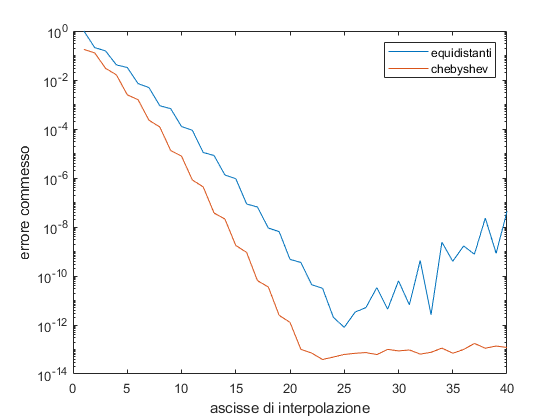
\includegraphics[scale=0.8]{CodiceMatlab/Esercizio15-19/graficoEs15.png}
    \caption{Grafico esercizio 15 con newton}
    \label{fig:es15}    
\end{figure}


\begin{figure}[h!]
    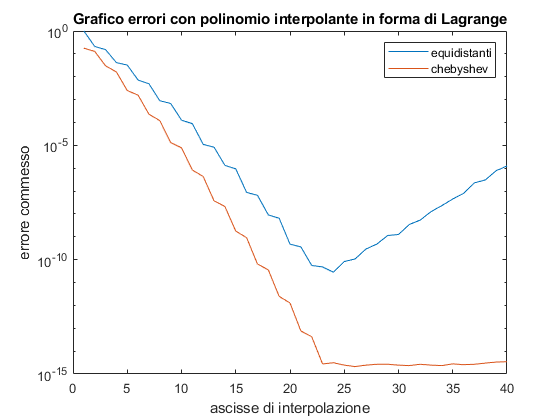
\includegraphics[scale=0.8]{CodiceMatlab/Esercizio15-19/graficoEs15Lagrange.png}
    \caption{Grafico esercizio 15 con Lagrange}
    \label{fig:es15}    
\end{figure}
Possiamo notare dal grafico 1  che l'errore nel caso delle ascisse di chebyshev è costantemente minore rispetto a quello delle ascisse equidistanti. Dopo n = 23  il grafico dell'errore commesso utilizzando le ascisse di chebyshev presenta un andamento costante. Per le ascisse equidistanti ( utilizzando i metodo di newton ) invece, l'errore raggiunge il valore minimo a n =25 , e  in seguito inizia a salire con un andamento non costante.\\
Possiamo notare che il grafico 2 è molto simile a quello precedente per quanto riguarda le ascisse di chebyshev. Mentre per le ascisse equidistanti, l'errore dopo aver raggiunto il suo valore minimo non presenta l'andamento a "zig zag".\\
Al crescere del numero delle ascisse di interpolazione l'errore commesso scegliendo le ascisse di chebyshev rimane più o meno costante in entrambi i casi. Questo è dovuto al fatto che la costante di Lebesgue equivale a circa $\frac{2}{\pi}\log{n}$, e risulta quindi avere una crescita ottimale, mentre per le ascisse equidistanti invece si ha una crescita esponenziale al crescere di n.

\section{Esercizio 16}
\begin{itemize}
\item Hermite
\lstinputlisting[language=Matlab]{CodiceMatlab/Esercizio15-19/hermite.m}
\item Script es. 16
\lstinputlisting[language=Matlab]{CodiceMatlab/Esercizio15-19/scriptEs16.m}
\end{itemize}
Eseguendo lo script si ottiene il seguente grafico: 

\begin{figure}[h!]
    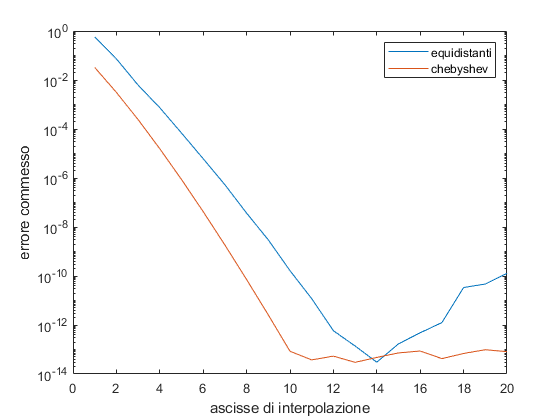
\includegraphics[scale=0.8]{CodiceMatlab/Esercizio15-19/graficoEs16.png}
    \caption{Grafico esercizio 16 con Hermite}
    \label{fig:es16}    
\end{figure}

Si può osservare che dopo n = 10  il grafico dell'errore per le ascisse di chebyshev  presenta un andamento costante. 
Per le ascisse equidistanti utilizzando il polinomio di Hermite l'errore raggiunge il valore minimo a n = 14 ed in seguito torna a salire.
Possiamo affermare che in generale l'approssimazione tramite ascisse di chebyshev è più precisa.

\section{Esercizio17}
\lstinputlisting[language=Matlab]{CodiceMatlab/Esercizio15-19/splinenat.m}
\section{Esercizio 18}
\lstinputlisting[language=Matlab]{CodiceMatlab/Esercizio15-19/scriptEs18.m}
Eseguendo lo script si ottiene il seguente grafico:
\begin{figure}[h]
    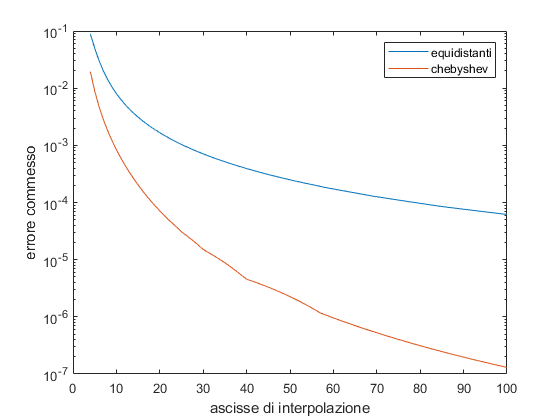
\includegraphics[scale=0.8]{CodiceMatlab/Esercizio15-19/graficoEs18.png}
    \caption{Grafico esercizio 18}
    \label{fig:es18}    
\end{figure}
\section{Esercizio19}
\lstinputlisting[language=Matlab]{CodiceMatlab/Esercizio15-19/scriptEs19.m}
Eseguendo lo script si ottiene il seguente grafico:
\begin{figure}[h]
    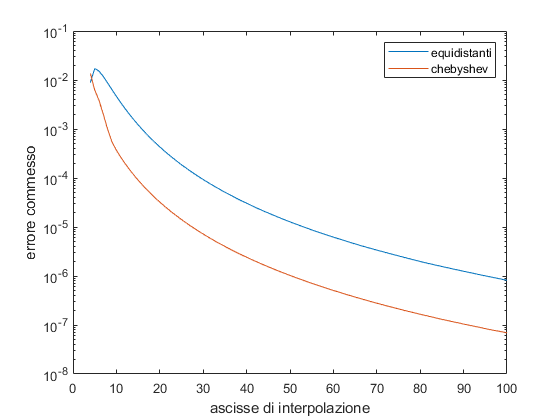
\includegraphics[scale=0.8]{CodiceMatlab/Esercizio15-19/graficoEs19.png}
    \caption{Grafico esercizio 19}
    \label{fig:es19}    
\end{figure}

Confrontando i due grafici possiamo notare che la funzione spline di Matlab commette un errore minore rispetto a splinenat. 
\begin{itemize}
\item Asisse di Chebyshev
 I grafici presentano un'andamento molto simile formando una curva che parte da $10^{-2}$ a $10^{-7}$, essendo l'errore commesso dalla funzione spline leggermente minore.
\item Ascisse equidistanti
Dai grafici si può osservare che utilizzando ascisse equidistanti la funzione splinenat commente un'errore notevolmente maggiore rispetto alla funzione spline di Matlab: nel caso della splinenat l'errore varia da $10^{-1}$ a $10^{-4}$,mentre nel caso della spline di matlab l'errore varia da circa $10^{-2}$ a $10^{-6}$.
\end{itemize}
\section{Esercizio 20}
Polinomio di approssimazione ai minimi quadrati
\lstinputlisting[language=Matlab]{CodiceMatlab/Esercizio20/scriptEs20.m}
Eseguendo lo script si ottiene il seguente grafico:
\begin{figure}[h!]
    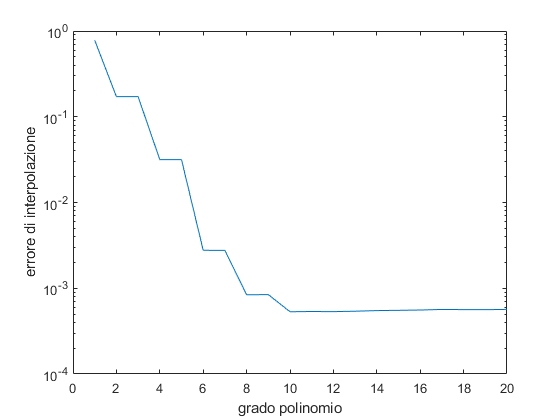
\includegraphics[scale=0.8]{CodiceMatlab/Esercizio20/graficoEs20.png}
    \caption{Grafico esercizio 20}
    \label{fig:es20}    
\end{figure}

Si può osservare  che l'errore decresce quasi esponenzialmente fino a circa $10^{-3}$, e quando il grado del polinomio m>=10, il grafico presenta un andamento costante.
\section{Esercizio 21}
\lstinputlisting[language=Matlab]{CodiceMatlab/Esercizio21-23/pesiNewtonCotes.m}
Di seguito sono riportati i valori dei pesi delle formule di newton cotes di grado n = 1....7 .

\begin{table}[ht]
	\centering
	\small
	\begin{tabular}{| c| c | c| c | c |  c |  c |  c | c |}
	\hline
	grado/cnk & 0& 1 &2 &3&4&5&6&7\\
	\hline
	1 & 1/2 & 1/2 & & & & & & \\
	\hline
	2 & 1/3& 4/3 &1/3 & & & & &  \\
	\hline
	3 & 3/8 & 9/8 & 9/8 & 3/8  & & & &\\
	\hline
	4 & 14/45 & 64/45 & 8/15 & 64/45 & 14/45 & & &\\
	\hline
	5 & 95/288 & 125/96 &125/144 &125/144&12/96&95/288 && \\
	\hline
	6 &41/140& 54/35 &27/140 &68/35&27/140&54/35 &41/140 &\\
	\hline
	7 & 1073/3527 & 810/559 & 343/640 &649/536 &649/536&343/640&810/559  &1073/3527\\
	\hline
	
	\end{tabular}
\end{table}

\section{Esercizio22}
\lstinputlisting[language=Matlab]{CodiceMatlab/Esercizio21-23/scriptEs22.m}
Eseguendo lo script si ottiene il seguente grafico:
\begin{figure}[h]
    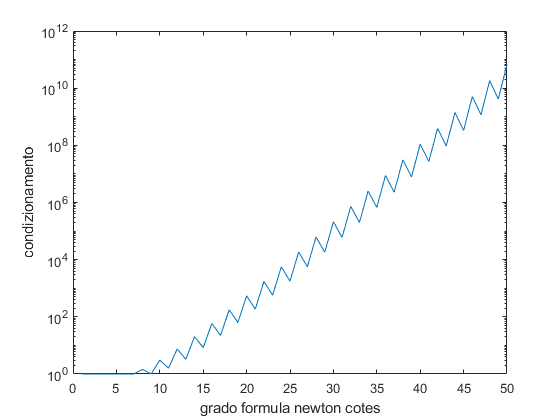
\includegraphics[scale=0.8]{CodiceMatlab/Esercizio21-23/graficoEs22.png}
    \caption{Grafico esercizio 22}
    \label{fig:es16}    
\end{figure}
\section{Esercizio 23}
Nella seguente tabella sono riportati i valori approssimati fino a 3 cifre significative in notazione scientifica.
\begin{table}[ht]
	\centering
	\small
	\begin{tabular}{| c| c | c|}
	\hline
	grado & approssimazione& errore\\
	\hline
	1 & 4.2800e-01 & 2.5300e-01\\
	\hline
	2 &2.1300e-01&3.8100e-02\\
	\hline
	3 & 1.9600e-01 & 2.1100e-02\\
	\hline
	4 & 1.8000e-01 &5.0800e-03\\
	\hline
	5 & 1.7900e-01&4.0800e-03  \\
	\hline
	6 &1.7600e-01&1.0800e-03 \\
	\hline
	7 & 1.7600e-01 & 1.0800e-03\\
	\hline
	8 & 1.7500e-01 &  7.8400e-05\\
	\hline
	9 & 1.7500e-01  &7.8400e-05\\
	\hline
	\end{tabular}
\end{table}
\section{Esercizio 24}
Sono state riportate solo le prime 10 iterazioni.

\begin{table}[ht]
	\centering
	\small
	\begin{tabular}{| c | c | c|}
	\hline
	Iterazioni & Trapezio & Simpson\\
	\hline
	2 & 2.664035584060345e-01&2.126315681335669e-01\\
	\hline
	4&2.034328044500163e-01&1.824425531313435e-01\\
	\hline
	6 &1.884983466139722e-01&1.773334438860330e-01\\
	\hline
	8&1.827894088752250e-01&1.759082770169613e-01\\
	\hline
	10&1.800348035219603e-01&1.753928683822888e-01 \\
	\hline
	12&1.785040157074719e-01&1.751725720719718e-01\\
	\hline
	14&1.775682181954108e-01&1.750665465192467e-01\\
	\hline
	16&1.769554131112014e-01&1.750107478565269e-01\\
	\hline
	18&1.765327096164695e-01&1.749792544399417e-01\\
	\hline
	20&1.762290375520298e-01&1.749604488953863e-01\\
	\hline
	\end{tabular}
\end{table}




\section{Esercizio 25}
\begin{itemize}
\item Simpson Adattiva
\lstinputlisting[language=Matlab]{CodiceMatlab/Esercizio25/adapsim.m}
\item Trapezi Adattiva
\lstinputlisting[language=Matlab]{CodiceMatlab/Esercizio25/adaptrap.m}
\item script
\lstinputlisting[language=Matlab]{CodiceMatlab/Esercizio25/scriptEs25.m}
\end{itemize}
Di seguito sono riportati i dati ottenuti:
\begin{table}[ht]
	\centering
	\small
	\begin{tabular}{| c | c | c| c | c | }
	\hline
	Tolleranza & Trapezio& N.Punti & Simpson & N. punti\\
	\hline
	$10^{-2}$ & 2.955597117841284e-01& 21 &2.812976430626699e-01&17\\
	\hline
	$10^{-3}$ &2.945853681850339e-01& 93 &2.812976430626699e-01&17\\
	\hline
	$10^{-4}$  &2.942742008736351e-01& 277 &2.942593384196308e-01&41\\
	\hline
	$10^{-5}$ &2.942301421648779e-01& 793 & 2.942278097680047e-01&81\\
	\hline
	$10^{-6}$ &2.942260196031783e-01& 2693&2.942257646203842e-01&145\\
	\hline
	\end{tabular}
\end{table}
\\$\int_{-1}^{1} \frac{1}{1+10^2x^2}  dx =0.29423$ ( circa ).\\
\\
Dai dati riportati in tabella risulta che entrambe le funzioni calcolano un'approssimazione molto precisa dell'integrale.\\
Inoltre,si nota immediatamente che la formula adattiva di Simpson calcola l'approssimazione dell'integrale utilizzando un numero di punti  nettamente inferiore  rispetto a quella del Trapezio.Il costo computazionale in questo caso dipende dal numero di chiamate ricorsive effettuate ( cioè di punti  calcolati ) , per cui possiamo affermare che  la formula adattiva di Simpson è più efficiente rispetto a quella del Trapezio.
\end{document}